\chapter{Background}

\section{Introduction to Remote Sensing}
Remote sensing (RS) is commonly defined as the acquisition of information about an object through sensors without direct physical contact. This information is obtained by detecting and measuring the modifications the object induces in its surrounding fields, which may include electromagnetic, acoustic, or potential fields \cite{book_Physics_Techniques_RS}.

RS is a relatively recent scientific discipline characterized by its strong interdisciplinary nature. It draws upon a wide spectrum of fields, requiring practitioners to develop a broad foundational understanding of both natural and applied sciences. Effective research in remote sensing often involves collaboration with specialists in electromagnetic theory, spectroscopy, applied physics, geology, atmospheric sciences, oceanography, electrical engineering, and optical engineering \cite{book_Physics_Techniques_RS}.

Remote observations require an interaction of energy between the target and the sensor. In the case of passive sensors, the detected energy originates from external or natural sources, such as solar radiation reflected by the Earth's surface or thermal radiation emitted by the object itself. A prominent example is the \textit{Landsat} program \footnote{https://landsat.gsfc.nasa.gov/}, which represents the longest continuously operating Earth observation mission. Over several decades, Landsat has generated a continuous global record, contributing significantly to environmental monitoring and Earth system science.

By contrast, active sensors generate their own energy pulses to illuminate the target and subsequently measure the portion of the signal that is reflected or backscattered. This capability allows them to operate independently of solar illumination and under a wide range of environmental conditions, including day or night and, in the case of microwave systems, through cloud cover and adverse weather \cite{RS_platforms_survey}. The most widely used active sensing technologies are Radar (Radio Detection and Ranging), which transmits and receives microwave radiation, and LiDAR (Light Detection and Ranging), which employs laser pulses in the optical domain. Both systems record the properties of the reflected signals to extract information about the target.

The term \textit{Remote Sensing} was introduced in the early 1960s to denote techniques for observing the Earth from a distance, with particular reference to aerial photography, which represented the predominant sensing technology at that time \cite{book_Satellite_RS}.

With the advent of satellites, global and synoptic observations of Earth and other planetary environments have become possible. Earth-orbiting sensors provide essential data on atmospheric dynamics, cloud distribution, vegetation cover, and its seasonal variability. Their long-term operation and repetitive coverage enable the monitoring of rapidly changing processes, such as polar ice dynamics and tropical deforestation. Beyond Earth, planetary missions (orbiters, flybys, landers, and rovers) have extended similar observations to all major planets in the solar system. To date, every planet has been visited at least once \cite{book_Physics_Techniques_RS}.
% \newpage

The origins of remote sensing date back to the invention of photography in 1839, which soon after was applied to topographic mapping. By the mid-19th century, aerial photographs were obtained from balloons, followed later by kites, pigeons, and eventually airplanes—the latter marking a decisive step with Wilbur Wright's first aerial photographs in 1909. Aerial photography became essential during World War I and advanced further in the 1930s-1940s with the introduction of color and infrared-sensitive films, widely used during World War II for reconnaissance and camouflage detection \cite{book_Physics_Techniques_RS,book_Satellite_RS}.

\begin{figure}[H]
  \centering
  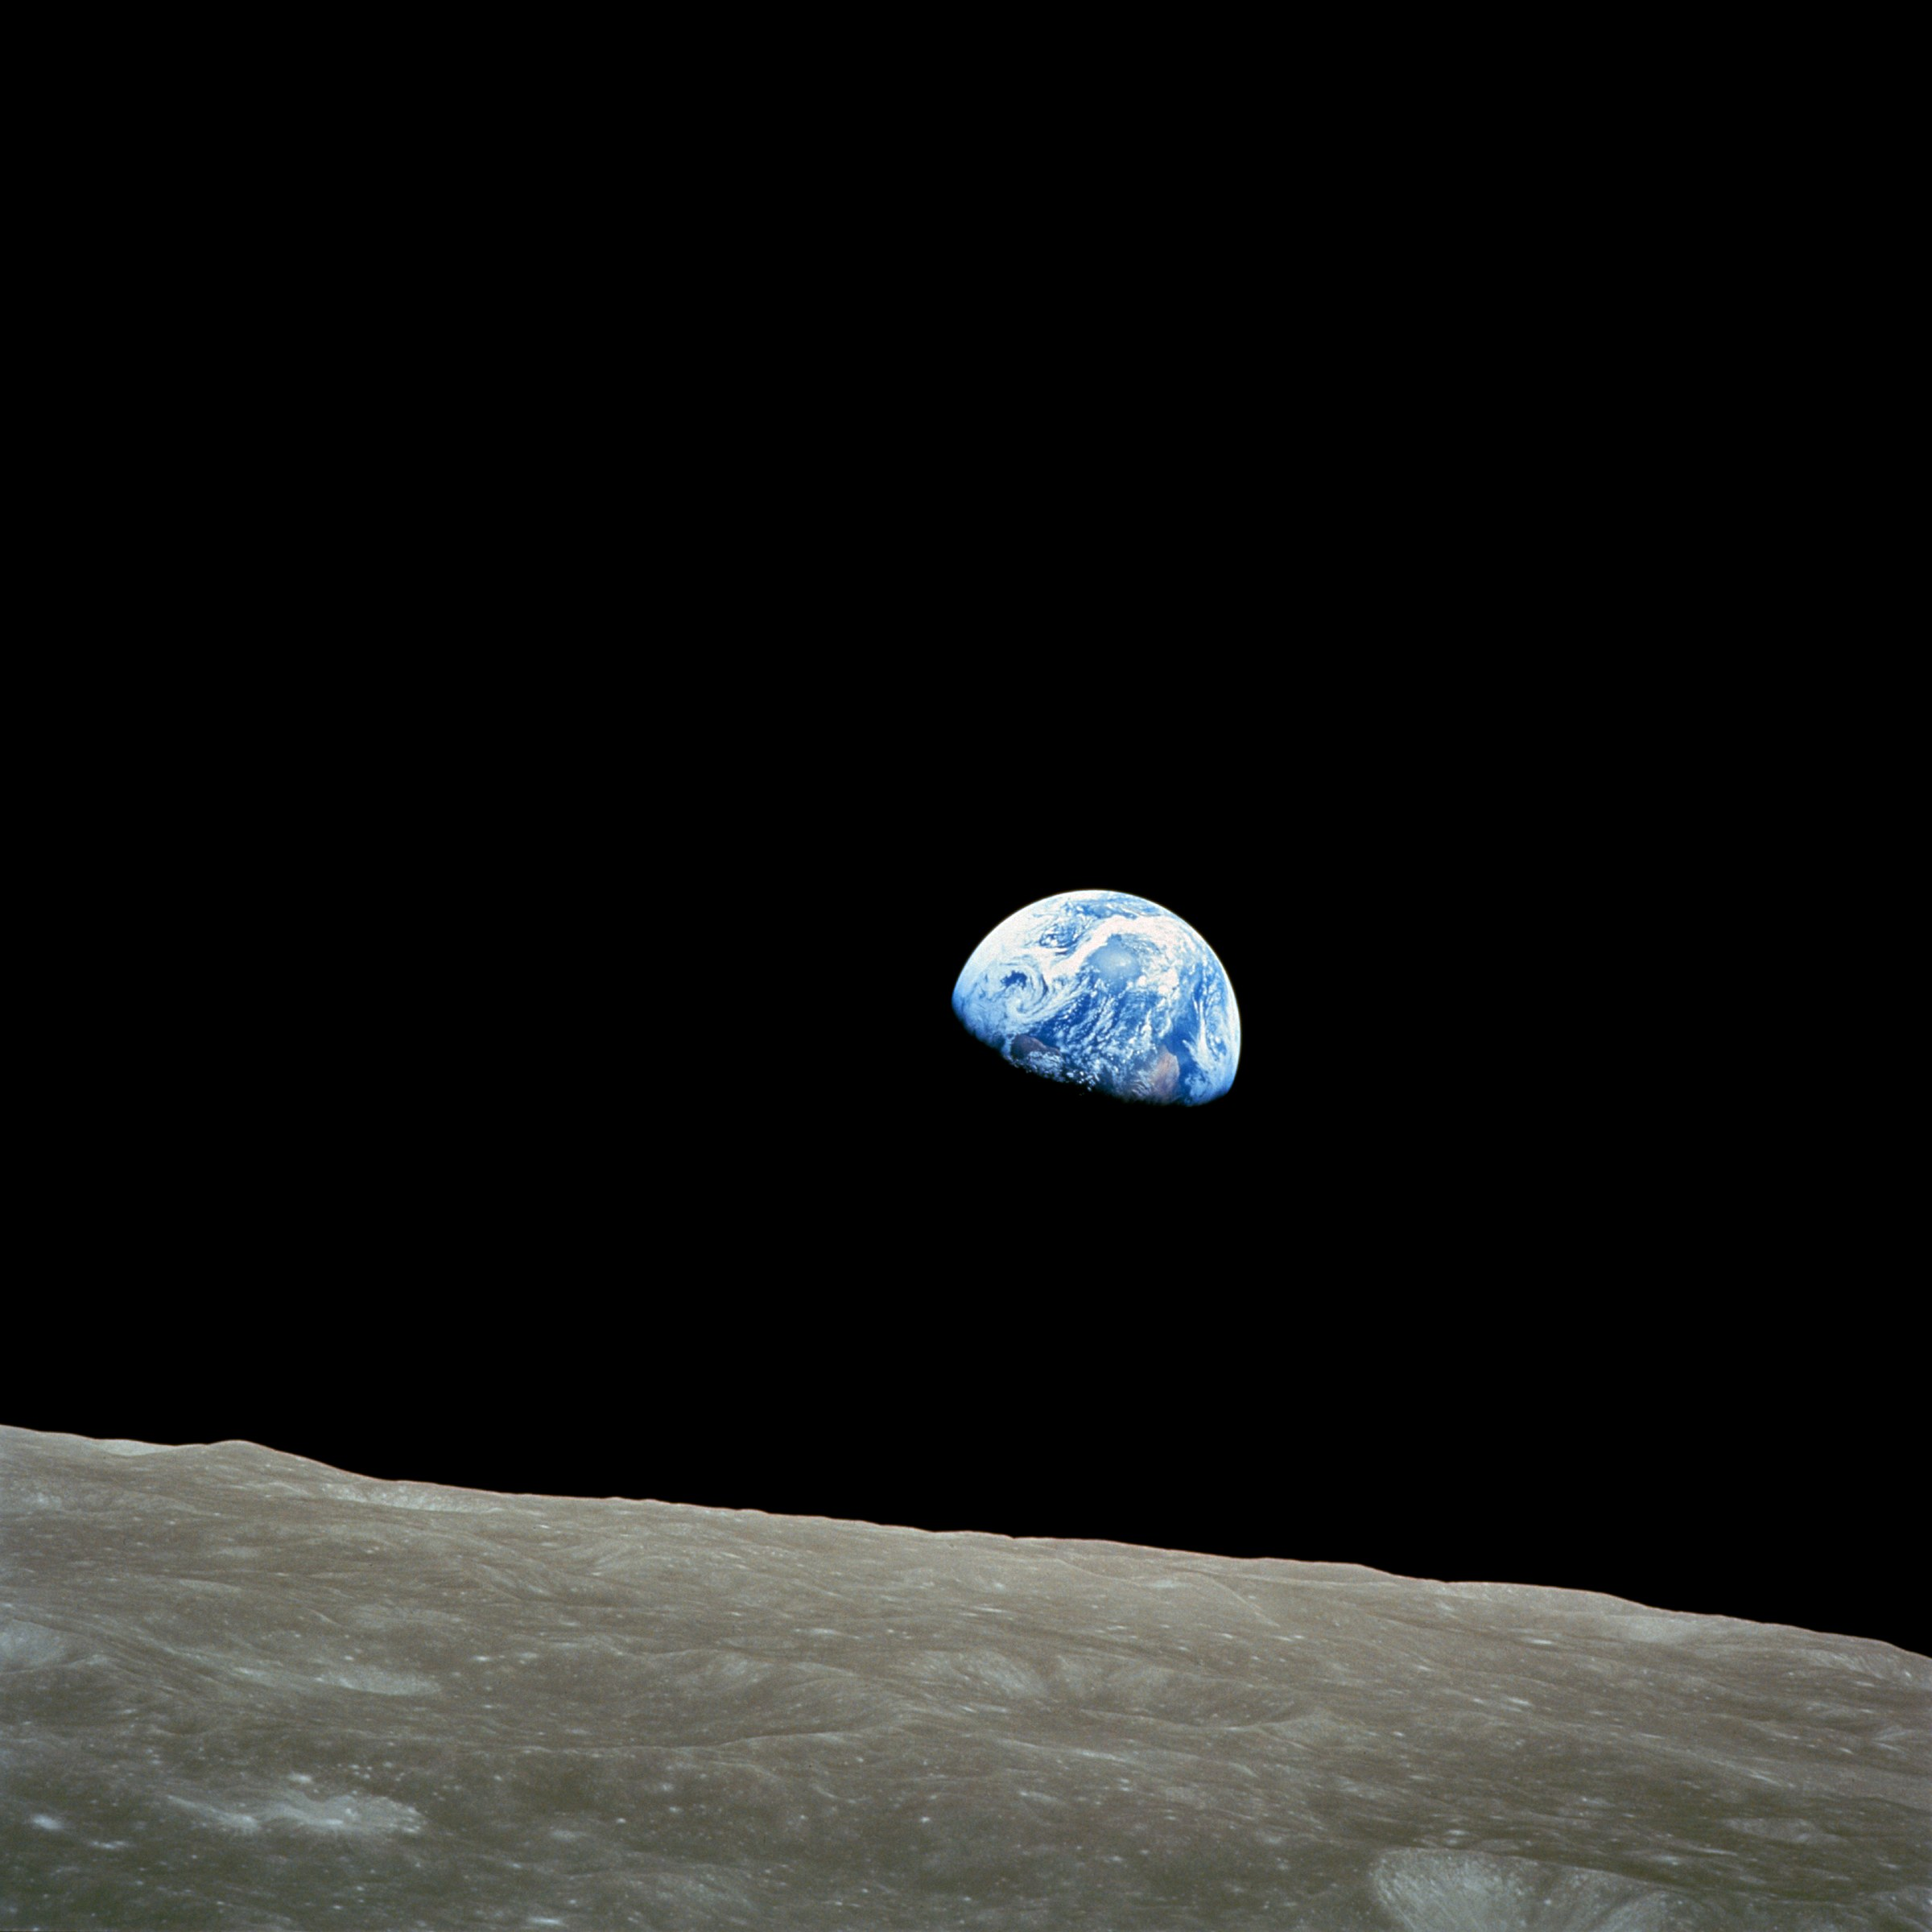
\includegraphics[width=0.95\textwidth]{img/earthrise.jpg}
  \caption{The iconic “Earthrise” photograph taken by astronaut William Anders during the Apollo 8 mission in 1968. Source: NASA.}
  \label{fig:earthrise}
\end{figure}

The postwar decades brought rapid technological progress with the development of radar and synthetic aperture radar (SAR), enabling high-resolution imaging independent of daylight or weather. Early rocket experiments in the late 1940s foreshadowed the space age, initiated by the launch of Sputnik in 1957. NASA's TIROS-1 satellite (1960) delivered the first global meteorological observations, while the launch of Landsat-1 in 1972 introduced systematic multispectral Earth observation, a program that continues today as the longest-running record of land surface change \cite{book_Physics_Techniques_RS,book_Satellite_RS}.

A symbolic milestone came with the Apollo 8 mission in 1968, when astronaut William Anders captured the famous Earthrise photograph, showing Earth rising above the lunar horizon (see Figure \ref{fig:earthrise}). This image not only had profound cultural, philosophical, and scientific impact but also highlighted the scientific value of spaceborne Earth observation.

Since the 1980s, remote sensing has expanded through international efforts such as SPOT (France, 1986), MOS-1 (Japan, 1987), and IRS-1 (India, 1988). The European Space Agency (ESA) \footnote{https://www.esa.int/} launched its first radar satellite, ERS-1, in 1991, and a second with comparable specifications in 1995. The 1990s and 2000s saw the rise of commercial satellites like IKONOS and QuickBird, offering very high-resolution imagery. Today, constellations of small satellites operated by private companies provide near-daily global coverage at meter-scale resolution. These advances—driven by improvements in optics, sensors, data transmission, and digital processing—have transformed remote sensing into a cornerstone of Earth system science, environmental monitoring, disaster response, and planetary exploration \cite{book_Satellite_RS}.

A summary of major milestones in the historical development of remote sensing platforms, from early balloon photography to modern satellite constellations, is illustrated in Figure~\ref{fig:RS_timeline}.

\begin{figure}[H] % requires \usepackage{float}
  \centering
  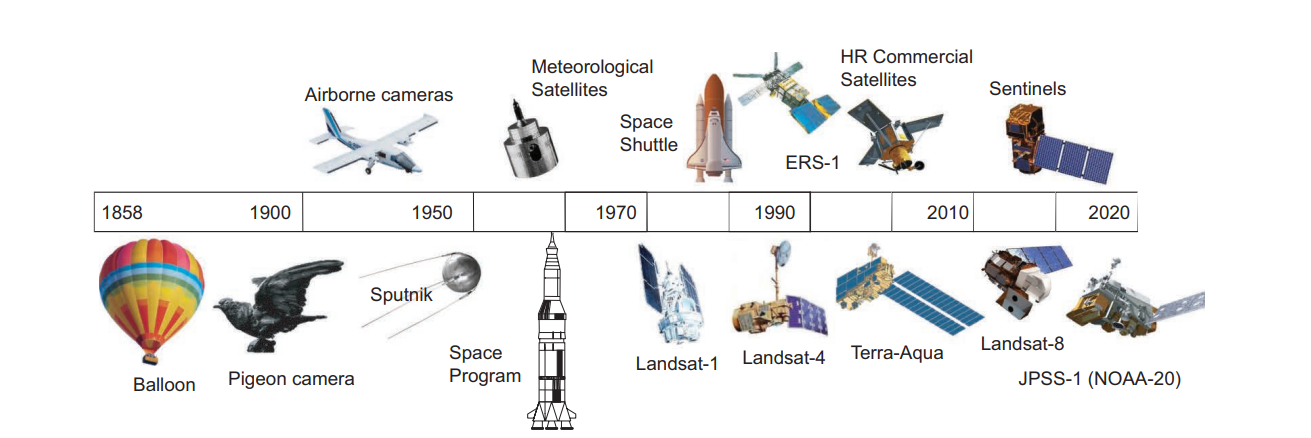
\includegraphics[width=\textwidth]{img/RS_timeline.png}
  \caption{Timeline of remote sensing platform development, from early airborne cameras to modern Earth observation satellites. Adapted from \cite{book_Satellite_RS}.}
  \label{fig:RS_timeline}
\end{figure}


\section{Copernicus: Europe's eyes on Earth}
Copernicus, known as the most ambitious Earth observation programme, is the Earth observation component of the European Union's Space Programme.
It is funded, coordinated, and managed by the European Commission in cooperation with partners such as the European Space Agency (ESA) and the European Organisation for the Exploitation of Meteorological Satellites (EUMETSAT)\footnote{https://www.eumetsat.int/}. The programme was named after the European scientist and observer Nicolaus Copernicus\footnote{https://www.biography.com/scientists/nicolaus-copernicus}. It integrates satellite and in situ observations (e.g., ground stations, airborne and seaborne instruments) to provide reliable, up-to-date information. Its services cover six domains: land, marine, atmosphere, emergency management, security, and climate change. 

The Copernicus Space Component features a new family of dedicated satellites,
called Sentinels, depicted in Figure \ref{fig:sentinels}, specifically designed for the operational needs of the Copernicus programme. 

\begin{figure}[H]
  \centering
  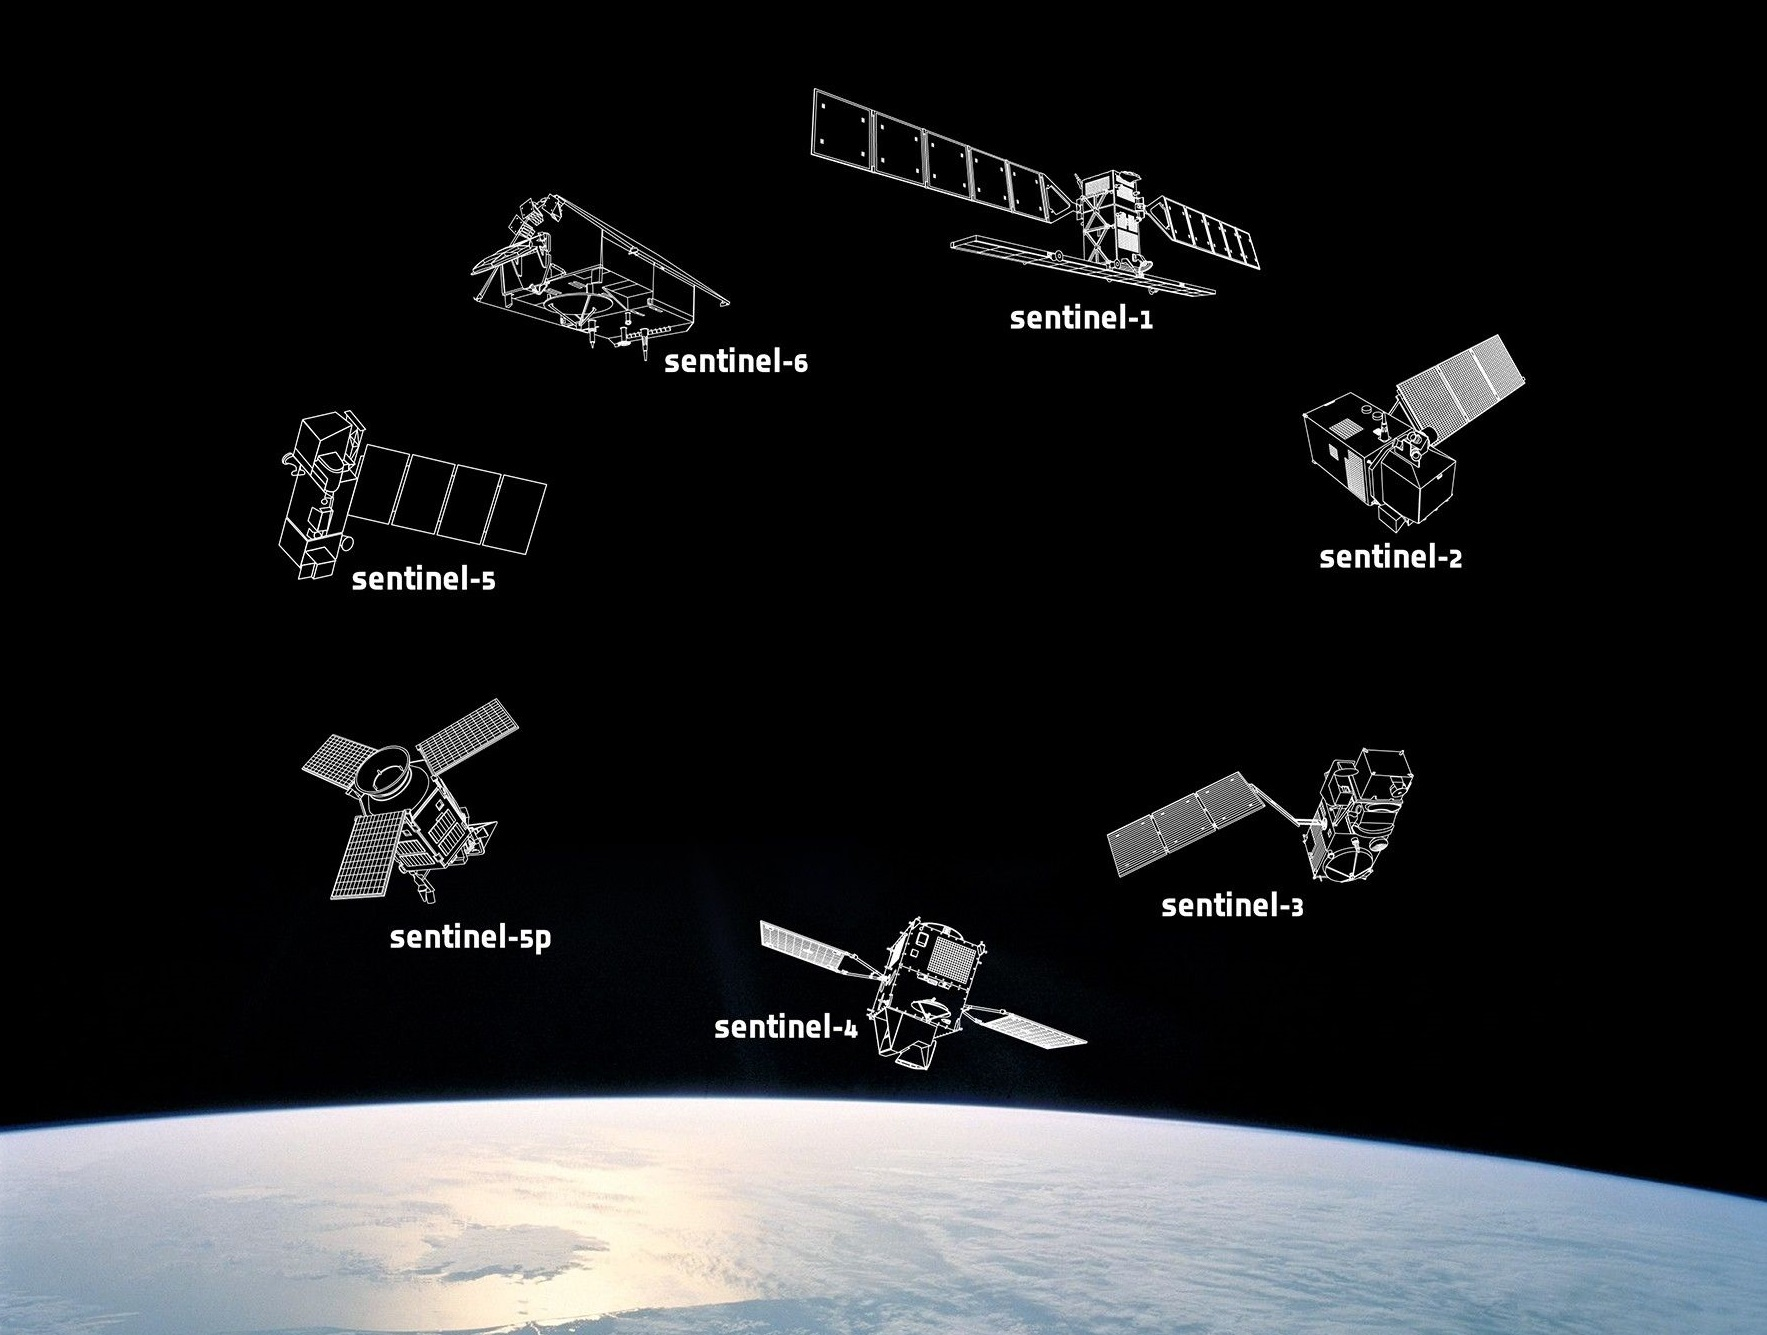
\includegraphics[width=0.95\textwidth]{img/sentinels.png}
  \caption{An artist's impression of the Copernicus Sentinel Missions. Source: ESA.}
  \label{fig:sentinels}
\end{figure}

On 3 April 2014, the deployment of the Copernicus Space Component began with the
launch of the \textsc{Sentinel-1} radar satellite, operating in the C-band and providing all-weather, day-and-night radar imagery. It was followed by its radar successors in 2016 and 2024. Its synthetic aperture radar (SAR) instruments are crucial for monitoring land deformation, subsidence, sea-ice dynamics, and emergency situations such as flooding and earthquakes \cite{ESA_Copernicus,ESA_SentinelMissions}.

\textsc{Sentinel-2}, launched in 2015, 2017, and 2024, is designed to deliver high-resolution, multispectral optical images, supporting applications such as agriculture, forestry, land use, disaster management, and climate studies. Its 13 spectral bands enable detailed analysis of vegetation health, water quality, and land cover dynamics \cite{ESA_Copernicus}.

The two \textsc{Sentinel-3} satellites, launched on 16 February 2016 and 25 April 2018, provide data for services relevant to the ocean and land. They carry instruments to measure sea surface topography, sea and land surface temperature, and ocean and land colour, providing essential data for oceanography, marine resource management, and climate monitoring \cite{ESA_SentinelMissions,ESA_Copernicus}.

\textsc{Sentinel-4} is an ultraviolet, visible, and near-infrared spectrometer carried on the Meteosat Third Generation Sounder satellites. Launched on 1 July 2025, it is dedicated to monitoring atmospheric composition and air quality over Europe and parts of North Africa. It provides hourly measurements of key trace gases and aerosols, enabling near-real-time assessments of air pollution, UV radiation, and climate-relevant processes \cite{ESA_Copernicus}.

Launched on 13 October 2017, the \textsc{Sentinel-5P} mission (Sentinel-5 Precursor) is the first Copernicus mission dedicated to monitoring the atmosphere. It provides high spatio-temporal resolution data for air quality, ozone and UV radiation, as well as climate monitoring and forecasting \cite{ESA_SentinelMissions}.

\textsc{Sentinel-6} is dedicated to high-precision ocean monitoring, focusing on sea surface topography. It continues the long-term record of satellite altimetry, measuring global sea level rise and ocean circulation patterns. These data are critical for climate change research, weather forecasting, and operational oceanography. Sentinel-6 was launched on 21 November 2020 \cite{ESA_SentinelMissions}. 

Looking into the future, six Sentinel Expansion missions will join the fleet. These include, among others, the Hyperspectral Imaging Mission, the Polar Ice and Snow Topography Altimeter, and the Anthropogenic Carbon Dioxide Monitoring mission \cite{ESA_Copernicus}.

Since the focus of this work is on SAR and Optical data, only Sentinel-1 and 2 will be discussed in details in the next sections. 

\subsection{Sentinel-1}

\subsection{Sentinel-2}



\newpage
\section{Data Availability and Limitations}

\subsection{Focus: Cloud Removal}

\subsection{Other Challenges}

\section{Generative AI}
\subsection{Pre-GenAI: Classical Approaches}
\subsection{Deep Learning and Computer Vision}
\subsection{Generative Adversarial Networks (GANs)}
\subsection{Diffusion Models}
\subsection{Vision Transformer}
\subsection{Vision Mamba}

\section{Application and Relevance to KIWA}


